%% This is an example first chapter.  You should put chapter/appendix that you
%% write into a separate file, and add a line \include{yourfilename} to
%% main.tex, where `yourfilename.tex' is the name of the chapter/appendix file.
%% You can process specific files by typing their names in at the 
%% \files=
%% prompt when you run the file main.tex through LaTeX.
\newenvironment{mylisting}
{\begin{list}{}{\setlength{\leftmargin}{1em}}\item\scriptsize\bfseries}
{\end{list}}

\chapter{Overcoming Nondeterminism in Linux services}
This chapter first broadly summarizes the sources of nondeterminism
in Linux services discovered through our experiments (Section \ref{ch3:sources}).
Next, it explains the dynamic instrumentation techniques
we used to simulate deterministic execution (Section \ref{ch3:simulation})
and our results (Section \ref{ch3:data}).
Finally, it discusses some of the limitations 
of our approach to deterministic execution (Section \ref{ch3:issues}).

\section{Sources of Nondeterminism} \label{ch3:sources}
In this section, we describe the sources of nondeterminism
discovered using the data collection scheme
described in Chapter \ref{ch:boot}.
This study of nondeterminism reveals
subtle interactions between user-mode
applications, commonly used system libraries (e.g. the \texttt{libc} library),
the Linux operating system and the external world.
While our results are derived from analyzing a small
set of complex programs, they include
all sources of application-level nondeterminism that 
have been described in literature. Unlike existing work,
however, we cover the various interfaces between user-mode programs
and the Linux kernel in considerable detail.

\subsection{Linux Security Features} \label{ch3:security}
\noindent {\bf Address Space Layout Randomization (ASLR)} \newline
Address Space Layout Randomization (ASLR) involves random arrangement of
key memory segments of an executing program. When ASLR is enabled,
virtual addresses for the base executable, shared libraries, 
the heap, and the stack are different every time the program is run.
ASLR hinders several kinds of security attacks in which attackers have to predict
program addresses in order to redirect execution (e.g. \emph{return-to-libc} attacks). 
As mentioned earlier, two execution traces of even a
simple one-line program in $C$ are almost entirely different
when ASLR is enabled because of differences in
instruction and memory addresses. \newline

\noindent {\bf Canary Values and Stack Protection} \newline
Copying a \emph{canary} -- a dynamically chosen global value -- onto the
stack before each function call can help detect buffer overflow attacks, because 
an attack that overwrites the return address will also overwrite
the copy of the canary. Before a \texttt{ret}, a simple comparison 
of the global (and unchanged) canary
value with the (possibly changed) stack copy can prevent a buffer overflow attack.

In 32-bit Linux distributions, the $C$ runtime library, 
\texttt{libc}, provides a canary value in \texttt{gs:0x14}.
If Stack Smashing Protection (SSP) is enabled on compilation,
\texttt{gcc} generates instructions that use the canary value
in \texttt{gs:0x14} to detect buffer overflow attacks.
Because Pin gets control of the application before \texttt{libc}
initializes \texttt{gs:0x14}, multiple execution traces of a program
will diverge when \texttt{gs:0x14} is initialized and subsequently
read.  The manner in which the canary value in \texttt{gs:0x14} is initialized
depends on the \texttt{libc} version.
If randomization is disabled, \texttt{libc} will store a fixed
terminator canary value in \texttt{gs:0x14}; this does not lead to any nondeterminism.
When randomization is enabled, however,  
some versions of \texttt{libc} store an unpredictable value in \texttt{gs:0x14} 
by reading from \texttt{`/dev/urandom'}
or by using the \texttt{AT\_RANDOM} bytes provided by the kernel (see
Section \ref{ch3:rand}). 

\newpage
\noindent {\bf Pointer Encryption} \newline
Many stateless APIs return data pointers to clients 
that the clients are supposed to simply supply as arguments
to subsequent function calls. 
For instance, the \texttt{setjmp} and \texttt{longjmp} functions
can be used to implement a try-catch block in $C$: \texttt{setjmp} uses 
a caller-provided, platform-specific \texttt{jmp\_buf} structure
to store important register state that \texttt{longjmp} 
later reads to simulate a return from \texttt{setjmp}.
Since the \texttt{jmp\_buf} instance is accessible to clients of \texttt{setjmp}
and \texttt{longjmp}, it is possible that the clients may advertently or inadvertently
overwrite the return address stored in it and simulate a buffer-overflow attack
when \texttt{longjmp} is called.

Simple encryption schemes can detect mangled data structures.
For instance, in 32-bit Linux, \texttt{libc} provides
a {\em pointer guard}  in \texttt{gs:0x18}. 
The idea behind the pointer guard is the following: 
to encrypt a sensitive address $p$, a program
can compute $s = p$  $\oplus  $ \texttt{gs:0x18}, 
optionally add some bit rotations, and store it in a structure
that gets passed around. Decryption can simply invert any bit rotations, 
and then compute $p = s$ $\oplus  $ \texttt{gs:0x18} back. 
Any blunt writes to the structure from clients will be detected because
decryption will likely not produce a valid pointer. 
Pointer encryption is a useful security feature for some APIs
and is used by some versions of \texttt{libc} to protect addresses stored in \texttt{jmp\_buf}
structures.

This pointer guard has different values
across multiple runs of a program, just like the \texttt{libc} canary
value. Initialization of the \texttt{libc} pointer guard can 
therefore be a source of nondeterminism in program execution. 
In some versions of \texttt{libc}, the value of \texttt{gs:0x18} is the same
as the value of \texttt{gs:0x14} (the canary). In others,
the value of \texttt{gs:0x18} is computed by \texttt{XOR}ing \texttt{gs:0x14} with 
a random word (e.g. the return value of the \texttt{rdtsc} x86 instruction),
or reading other \texttt{AT\_RANDOM} bytes provided by the kernel
 (Section \ref{ch3:rand}).

\subsection{Randomization Schemes} \label{ch3:rand}
As already clear from Section \ref{ch3:security}, 
randomization schemes can lead to significant nondeterminism 
in programs. Applications generally employ pseudorandom number generators (PRNGs)
and rely on the PRNG seeds to differ across multiple program executions 
to generate truly random values. PRNG seeds are usually
computed from external sources:

\begin{itemize}
\item {\em The} \texttt{`/dev/urandom'}{\em special file}: Linux allows
running processes to access a random number generator through this
special file. The entropy generated from environmental noise (including
device drivers) is used in some implementations for the kernel random number generator.

\item \texttt{AT\_RANDOM} {\em bytes}: 
Using \texttt{open}, \texttt{read} and \texttt{close} system-calls 
to read only a few random bytes from \texttt{`/dev/urandom'} 
can be computationally expensive. 
To remedy this, some 
recent versions of the Linux kernel supply
a few random bytes to all executing programs
through the \texttt{AT\_RANDOM} auxiliary vector.
ELF auxiliary vectors are pushed on the program
stack below command-line arguments and environmental
variables before a program starts executing.

\item {\em The} \texttt{rdtsc} {\em instruction}:
The \texttt{rdtsc} instruction provides an approximate number of ticks since
the computer was last reset, which is stored in a 64-bit register present
on x86 processors. Computing the difference between two successive
calls to \texttt{rdtsc} can be used for timing, whereas a single
value returned from \texttt{rdtsc} lacks any useful context.  
The instruction has low-overhead, which makes it suitable for generating a random value
instead of reading from \texttt{`/dev/urandom'}. 

\item {\em The current time or process ID}: Many applications simply make a system call
to get the current time or the current process ID, 
and use the returned value to seed their PRNGs. 

\item {\em Miscellaneous}: There
are several creative ways to seed random number
generators (e.g. reading from {\em www.random.org}),
but we have not observed them
in our analysis of Linux services.
\end{itemize}

Thus, randomization-related nondeterminism in Linux services 
really originates from external sources used to seed PRNGs;
if the seeds are different across multiple
executions, PRNGs algorithms propagate this
nondeterminism.

\subsection{Process Identification Layer} \label{ch3:pid}
% pid, signal(pid), /proc/ filesystem layer

In the absence of a deterministic operating system layer, process IDs for
Linux services at boot-time are not predictable.
For instance, a nondeterministic scheduler (Section \ref{ch3:concurrency}) 
could lead to several possible process creation sequences
and, in turn, process ID assignments.

Given the unpredictability of process IDs,
system calls that directly or indirectly
interact with the process identification layer can cause divergences
in distinct executions of the same program.
For instance, system calls that return a process ID e.g.
\texttt{getpid} (get process ID), \texttt{getppid} (get
parent process ID), \texttt{fork/clone} (create a child process),
\texttt{wait} (wait for a child process to terminate)
can return different values across distinct executions. System calls that take process IDs 
directly as arguments such as \texttt{kill} (send a signal to a specific
process), \texttt{waitpid} (wait for a specific child process to terminate)
can similarly propagate any nondeterminism.
In fact, \texttt{libc} stores a copy of the current process ID in \texttt{gs:0x48},
so reads or writes to this address can cause conflicts.

Apart from system calls, there are other interfaces
between the Linux kernel and executing user-mode programs
where process IDs also show up:

\begin{itemize} 

\item {\em Signals}: If a process registers a signal handler with the \texttt{SA\_SIGINFO}
bit set, then the second argument passed
to the signal handler when a signal occurs is of type \texttt{siginfo\_t*}.
The member \texttt{siginfo\_t.si\_pid} will
be set if another process sent the signal 
to the original process (Section \ref{ch3:sig}). 

\item {\em Kernel messages}: The Linux kernel will sometimes use process IDs 
to indicate the intended recipients of its messages. 
For instance, \texttt{Netlink} is a socket-like
mechanism for inter process communications (IPC)
between the kernel and user-space processes.
\texttt{Netlink} can be used to pass
networking information between kernel
and user-space, and some of its APIs 
use process IDs to identify communication
end-points. (Section \ref{ch3:netio}). \end{itemize}

\newpage 
Nondeterminism arising from the unpredictability of process IDs can be
further propagated when an application uses process IDs to seed PRNGs 
(Section \ref{ch3:rand}), access the \texttt{`/proc/[PID]'} directory
(Section \ref{ch3:procfs}), name application-specific files or 
write to them. (Section \ref{ch3:fileio}). 

\subsection{Time} \label{ch3:time}
Concurrent runs of the same program will typically
execute the same instructions at (slightly) different times.
Clearly, any interactions of a program with timestamps
can cause nondeterminism. For instance:

\begin{itemize}
\item The \texttt{time}, \texttt{gettimeofday} and \texttt{clock\_gettime}
 system calls return the current time.
\item The \texttt{times} or \texttt{getrusage} system calls
return process and CPU time statistics respectively.
\item The \texttt{adjtimex} system call is used 
by clock synchronization programs (e.g. \texttt{ntp}) 
and returns a kernel timestamp indirectly via 
a \texttt{timex} structure.
\item Programs can access the hardware clock
through \texttt{`/dev/rtc'} and read the current time
through the \texttt{RTC\_RD\_TIME} \texttt{ioctl}
operation.
\item Many system calls that specify a timeout
for some action (e.g. \texttt{select}, \texttt{sleep} or \texttt{alarm})
inform the caller of any unused time from the timeout interval if they
return prematurely.
\item The \texttt{stat} family of system calls returns file
  modification timestamps; also, many application files typically contain timestamps;
  network protocols use headers with timestamps as well (Sections \ref{ch3:fileio}
  and \ref{ch3:netio}).
\end{itemize}

Apart from nondeterminism arising
from timestamps, {\em timing} differences
can arise between distinct executions 
because of variable system-call latencies 
or unpredictable timing of
external events relative
to program execution (Sections \ref{ch3:sig} and \ref{ch3:poll}).

\subsection{File I/O} \label{ch3:fileio}
\noindent {\bf File contents} \newline
If two executions of the same program read different
file contents (e.g. cache files), then
there will naturally be execution divergence.
However, for concurrently executing Linux services,
differences in file contents typically arise
from process IDs (Section \ref{ch3:pid}) or timestamps (Section \ref{ch3:time})
rather than semantic differences.
If those factors are controlled, file contents rarely differ. \newline

\noindent {\bf File Modification Times} \newline
Apart from minor differences in file contents,
nondeterminism can arise from distinct file 
modification (\texttt{mtime}), access (\texttt{atime}) or status-change (\texttt{ctime})
timestamps.
The \texttt{stat} system call is usually made for almost
every file opened by a program; the timestamps
in the buffer written by the system call invariably
conflict between any two executions. Most of the time,
these timestamps are not read by programs,
so there is little propagation. On occasion, 
however, a program will use these timestamps
to determine which file is more recent than another,
or whether a file has changed since
it was last read. \newline

\noindent {\bf File Size} \newline
When a program wishes to open
a file in append-mode, it uses \texttt{lseek}
with \texttt{SEEK\_END} to move
the file cursor to the end,
before any \texttt{write}s take place.
The return value of \texttt{lseek} is the
updated cursor byte-offset into the file.
Clearly, if the length of a file is different across
multiple exections of a program, then
\texttt{lseek} will return conflicting values.
Many Linux services maintain log files
which can have different lengths due
to conflicts in an earlier execution; \texttt{lseek}
further propagates them. To overcome
such nondeterminism, older log files
must be identical at the beginning 
of program execution and other
factors that cause nondeterminism
must be controlled. 

\newpage
Ultimately, however, if two input or configuration files
are semantically different between
different executions of a program, then 
execution will inevitably diverge. 

\subsection{Network I/O} \label{ch3:netio}
\noindent {\bf Network Configuration Files} \newline
The \texttt{libc} network initialization
code loads several configuration files
into memory (e.g. \texttt{`/etc/resolv.conf'}). 
Differences in the content, timestamps or lengths
of such configuration files can clearly cause nondeterminism.
Background daemons (e.g. \texttt{dhclient} for \texttt{`/etc/resolv.conf'}) 
usually update these files periodically in the background.
Calls to \texttt{libc} functions such as \texttt{getaddrinfo} use \texttt{stat} 
to determine if relevant configuration files (e.g. \texttt{`/etc/gai.conf'})
have been modified since they were last read. 
In our experiments, typically the file modification timestamps 
-- and not the actual contents -- of these configuration files 
vary between different executions,
because identical VMs have the same network setup
and behavior. \newline

\noindent {\bf DNS Resolution} \newline
In our experiments, IP addresses are resolved identically by concurrently executing services. 
However, if DNS-based load-balancing schemes are used, the same 
server can appear to have different IP addresses. \newline

\noindent {\bf Socket \texttt{read}s} \newline
Bytes read from sockets can differ between
executions for a variety
of reasons. For instance, different timestamps in 
protocol headers, or different requests/responses 
from the external world would be reflected in
conflicting socket \texttt{read}s.
By studying application behavior, it is possible
to distinguish between 
these different scenarios and
identify the seriousness
of any differences arising from socket reads.

In our experiments, we have only observed nondeterminism
in \texttt{read}s from \texttt{Netlink} sockets.
As mentioned in Section \ref{ch3:pid},
\texttt{Netlink} sockets provide a 
mechanism for inter-process communications (IPC)
between the kernel and user-space processes.
This mechanism can be used to pass
networking information between kernel
and user space. \texttt{Netlink} sockets
use process IDs to identify
communication endpoints, which can
differ between executions (Section \ref{ch3:pid}).
Some implementations of \texttt{libc} use
unpredictable timestamps to assign monotonically increasing sequence 
numbers to \texttt{Netlink} packets (Section \ref{ch3:time}).
Nondeterminism can also arise from sockets of the \texttt{NETLINK\_ROUTE}
family, which receive routing and link updates
from the kernel; \texttt{libc} uses \texttt{RTM\_NEWLINK}
messages to discover the link interfaces 
in the computer. When a new interface
is discovered or reported, the kernel supplies
interface statistics to \texttt{libc} 
such as packets sent, dropped or
received. These statistics will obviously vary
across different program instances.  \newline

\noindent {\bf Ephemeral Ports} \newline
A TCP/IPv4 connection consists of two end-points;
each end-point consists of an IP address and a port
number. An established client-server connection 
can be thought of as the
4-tuple (server\_IP, server\_port, client\_IP, client\_port).
Usually three of these four are readily known:
a client must use its own IP, and
the pair (server\_IP, server\_port) is fixed. What is not
immediately evident is that the client-side of 
the connection uses a port number.
Unless a client program explicitly
requests a specific port number,
an {\em ephemeral port} is used.
Ephemeral ports are temporary ports
assigned from a dedicated range by the machine IP stack,
When a connection
terminates, an ephemeral port can be recycled.
Since the underlying operating system
is not deterministic, ephemeral
port numbers used by Linux services
tend to be different across multiple 
runs. 

\subsection{Scalable I/O Schemes} \label{ch3:poll}
\noindent {\bf Polling Engines} \newline
Complex programs like Linux services have
many file descriptors open at a given time.
Apart from regular files, these file descriptors could correspond to:

\begin{itemize}

\item {\em Pipes}: Pipes are used for
  one-way interprocess communication (IPC).
  Many Linux services spawn child processes;
  these child processes communicate
  with the main process (e.g. for status
  updates) through these pipes.

\item A {\em listener socket}:
  If the program is a server,
  this is the socket that accepts incoming connections.

\item {\em Client-handler sockets}:
  If this program is a server, 
  new requests from already connected clients would arrive through
  such sockets.

\item {\em Outgoing sockets}:
  If the program is a client for other servers,
  it would use these sockets to send requests 
  to them.
\end{itemize}

The classic paradigm for implementing server
programs is {\em one thread or process per client}
because I/O operations are traditionally blocking
in nature. This approach scales poorly as the number
of clients -- or equivalently, the number of open file descriptors -- increases. 
As an alternative, event-based I/O is increasingly used 
by applications with many open file descriptors.
In event-based I/O, the event-thread
specifies a set of file descriptors it cares about,
and then waits for ``readiness'' notifications 
from the operating system on any of
these file descriptors by using a
system call such as \texttt{epoll}, \texttt{poll},
\texttt{select} or \texttt{kqueue}. 
For instance, a client socket would be ready 
for reading if new data was received from a client,
and an outgoing socket would be ready for 
writing if an output buffer was flushed out or if the 
connection request was accepted.
The event-thread invokes an I/O
handler on received event, 
and then repeats the loop to process the next
set of events.
This approach is often used for design simplicity because it
reduces the threads or processes needed by an application; 
recent kernel implementations (e.g. \texttt{epoll}) are also
efficient because they return the set of file descriptors that are ``ready'' for I/O,
preventing the need for the application to iterate through all its open
file descriptors. 

Event-based I/O can be a source
of nondeterminism in programs because the
timing of I/O events with respect to each other
can be different across multiple executions.
Even if I/O events are received in the same order,
the same amount of data may not be available
from ``ready'' file descriptors. Furthermore, when a timeout
interval is specified by the application for polling file descriptors,
\texttt{select} may be completed or interrupted
prematurely. In that case, \texttt{select} returns
the remaining time interval, which can     
differ between executions (Section \ref{ch3:time}). \newline

\noindent {\bf Asynchronous I/O Systems} \newline
Asynchronous I/O APIs (e.g. the Kernel Asynchronous I/O interface
in some Linux distributions) allow even a single application
thread to overlap I/O operations with other processing
tasks. A thread can request an I/O operation (e.g. \texttt{aio\_read}),
and later query the OS or be notified by it that the I/O operation
has been completed (e.g. \texttt{aio\_return}). While such APIs are in limited
usage, they would create nondeterminism because of the
variable absolute and relative timing of I/O events.

\subsection{Signals}\label{ch3:sig}
A signal is an event generated by Linux
in response to some condition, which may cause
a process to take an action in response.
Signals can be generated by error conditions
(e.g. memory segment violations), 
terminal interrupts (e.g. from the shell), 
inter-process communication (e.g. parent 
sends \texttt{kill} to child process),
or scheduled \texttt{alarm}s. 
Processes register handlers (or function callbacks) for specific signals
of interest, in order to respond to them.

Signals are clearly external to
instructions executed by a single process,
as such, they create nondeterminism 
much the same way as asynchronous I/O.
Signals can be delivered to multiple executions
of the same program in different order.
Even if signals are received in the
same order between different executions,
they can be received at different times
into the execution of a program.

\subsection{Concurrency} \label{ch3:concurrency}
Multiple possible instruction interleavings of 
threads within a single program, 
or of different processes within 
a single operating system are
undoubtedly significant sources
of nondeterminism.
Nondeterminism due to
multi-threading has been extensively
documented, and can cause
significant control flow differences
across executions.

Nondeterminism in the system
scheduler is external to 
program execution, and manifests itself
in different timing or ordering
inter-process communications (e.g.
through pipes, signals, or 
values written to file system logs).

\subsection{{\em Procfs}: The `/proc/' directory}\label{ch3:procfs}
Instead of relying on system-calls, user-space programs
can access kernel data much more easily using {\em procfs}, a hierarchical 
directory mounted at \texttt{`/proc/'}.
Procfs is an interface
to kernel data and system information
that would otherwise be available
via system calls (if at all);
thus, many of the sources of nondeterminsm
already described can be propagated
through it.

For instance, \texttt{`/proc/uptime'} contains time statistics about how
long the system has been running;
\texttt{`/proc/meminfo'} contains statistics about kernel memory management;
\texttt{`/proc/net/'} contains network statistics and IP addresses for interfaces;
\texttt{`/proc/diskstats/'} contains statistcs about any attached disks.
These files will differ across multiple executions
of a program because of nondeterminism in the underlying operating system. 

Apart from accessing system-wide information, a process can access 
information about its open file descriptors through
\texttt{`/proc/[PID]/fdinfo'} (e.g. cursor offsets and status).
Similarly, \texttt{`/proc/[PID]/status'} contains
process-specific and highly unpredictable statistics,
e.g. number of involuntary context switches,
memory usage, and parent process ID.
Performing a \texttt{stat} on files in \texttt{`/proc/[PID]/'}
will reveal process creation time.

\subsection{Architecture Specific Instructions}
Architecture specific instructions such as \texttt{rdtsc}
and \texttt{cpuid} can return different
results across program executions. As mentioned before
(Section \ref{ch3:rand}), the \texttt{rdtsc} instruction provides the number of ticks since
the computer was last reset, which
will differ across executions. The \texttt{cpuid} instruction
returns information about the processor and the underlying 
hardware, and its results can vary across different
executions as well.

\section{Simulating Deterministic Execution} \label{ch3:simulation}
We modified our data collection scheme from Chapter 2 (shown in Figure \ref{data:naive})
to simulate deterministic execution in the bootstorm scenario.

\begin{figure}[h]
  \center
  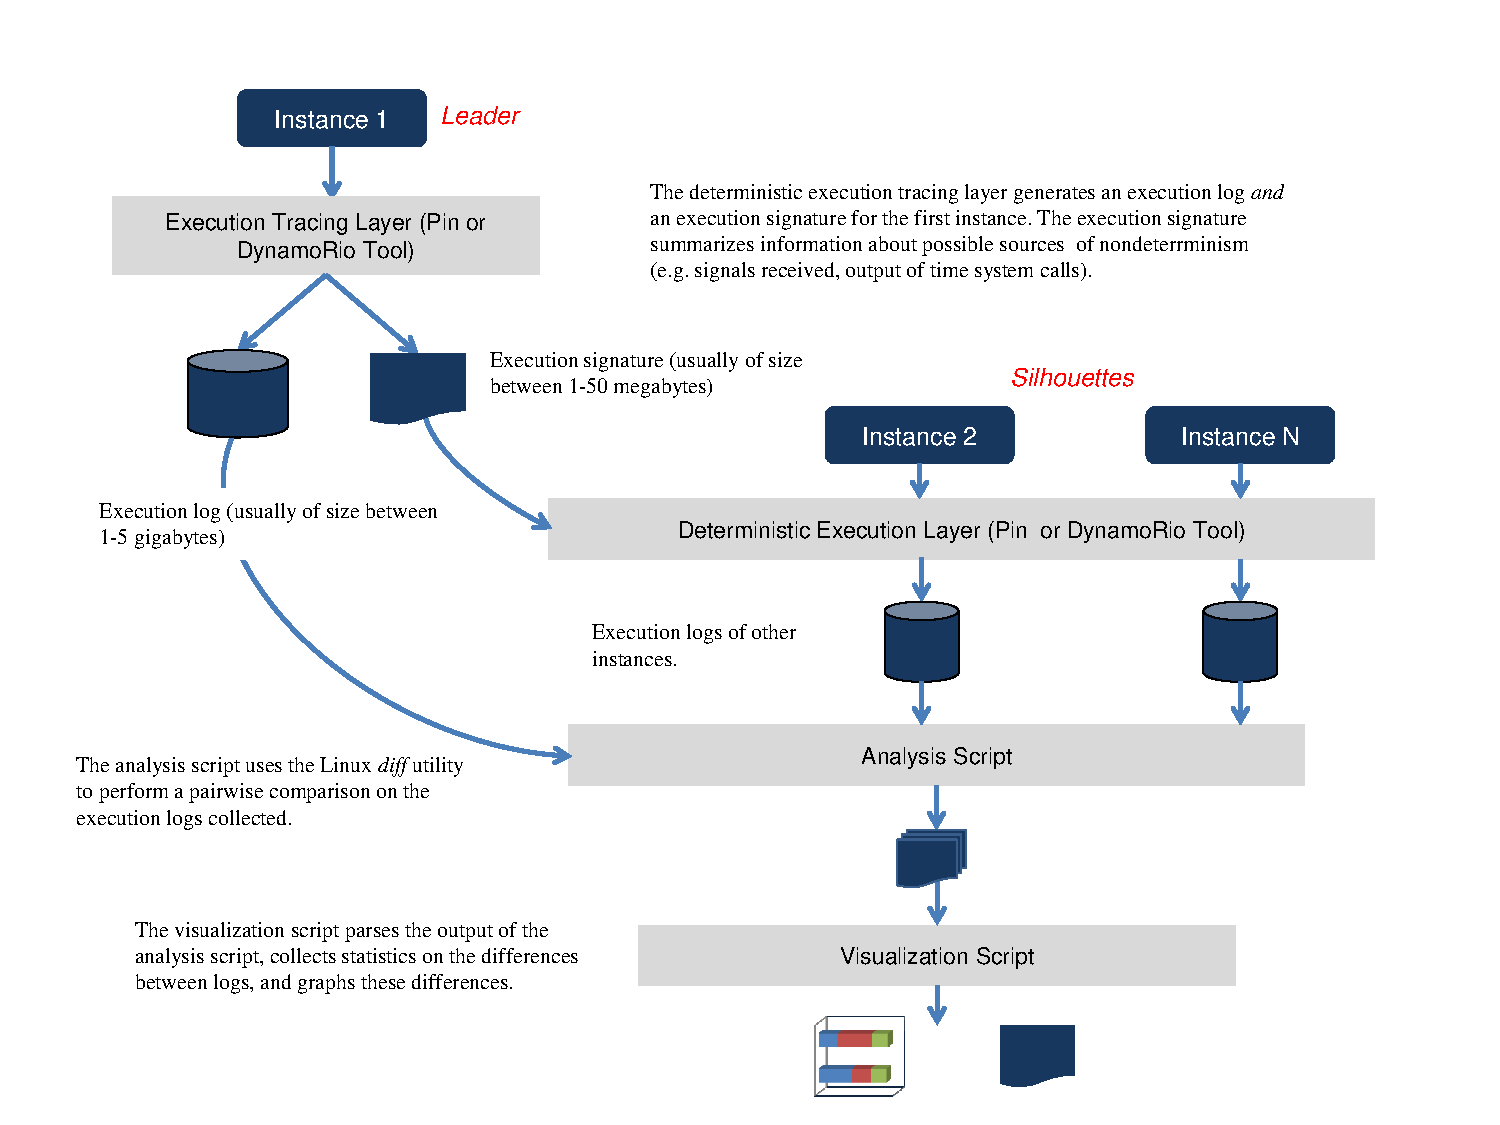
\includegraphics[scale=0.7, trim=1cm 0cm 1cm 0cm]
                  {simulation.pdf}
  \caption[Simulation of Deterministic Execution of Bootstorm scenario]%
  {Simulation of Deterministic Execution of Bootstorm scenario.}
  \label{ch3:figsimulation}
\end{figure}

As shown by Figure \ref{ch3:figsimulation}, we run one instance of the program before all others.
For this instance, we generate an {\em execution log}, as before,
but also summarize information about the sources of nondeterminism
described in Section \ref{ch3:sources}. For instance, we record
information about signal timing, process IDs, time-related system calls
in the {\em execution signature} file. Our dynamic instrumentation tool
uses the execution signature of the first instance 
to modify the instruction sequences executed by subsequently
executed instances, to boost determinism as much as possible.

This simulation scheme can be reconciled with possible solutions to the 
boot storm scenario that involve:
\begin{itemize}
\item
booting one VM before others,
then using its execution trace to {\em speed-boot} other VMs
in a less hardware-intensive manner, or
\item 
running VMs concurrently but with an assigned leader;
the VMs communicate with each other to overcome
nondeterminism.
\end{itemize}

In the first case, the execution signature file
conceptually represents the trace of the first VM used to speed-boot
other VMs. In the second case, it represents a log of the communications 
sent from the leader sent to concurrently booting VMs.
We now briefly describe how dynamic instrumentation can be used to overcome
the sources of nondeterminism described in \ref{ch3:sources}. \newline

\noindent {\bf Address Space Layout Randomization (ASLR)} \newline
Existing record-and-replay systems get around ASLR by
forcing the operating system to use the same address space layout across
different runs. A slightly more complicated approach would involve
using base/offset computations to translate equivalent 
addresses between two different executions. 
For our experiments, we simply disabled ASLR using the following command:
\texttt {sudo kernel.randomize\_va\_space=0} to simulate the 
case where multiple VMs nudge the operating system to construct
similar address spaces for the same process. \newline

\noindent {\bf Canary and Pointer Guard Values} \newline
Dynamic instrumentation can be used to force canary (\texttt{gs:0x14})
and pointer guard (\texttt{gs:0x18}) values
to agree across distinct executions of the same program:
instructions that initialize them can be
modified or replaced; the \texttt{AT\_RANDOM} bytes 
provided by the kernel can be
modified before they are read by the application; 
values read from \texttt{`/dev/urandom'} can be 
intercepted and modified; the \texttt{rdtsc} instruction can be emulated.
The execution signature file stores the canary and pointer guard values used by the first instance, 
and reuses them across other instances. \newline

\noindent {\bf Randomization and Time} \newline
To overcome nondeterminism resulting from randomization,
we need to intercept the standard techniques
used by programs to seed PRNGs.
As already mentioned, values read from \texttt{`/dev/urandom'}
or the \texttt{rdtsc} instruction can be easily replaced
using the execution signature file for the first instance.

Time-related system calls can
be intercepted in the same manner:
the timestamps logged
in the execution signature file
can be used to force agreement
between different executions.
For most time-related system calls,
high-fidelity replay is not necessary:
several timestamps generated
during program execution are simply ignored
(e.g. from \texttt{stat} calls),
so they can actually be replaced with any 
fixed value. Many timestamps
returned from system calls are only compared to
determine ``freshness'': they
can be replaced with deterministic ordinal values (e.g 0 or 1) that 
perserve the original comparison result.

Conceptually, these approaches simulate the possible but highly
unlikely case that all the instances of the same program
executed time-related system calls
at precisely the same times,
and several randomly generated values independently agreed. \newline

\noindent {\bf Signal Delivery} \newline
In order to overcome the unpredictable timing and 
order of signals, we intercept all signals received by 
an application and ensure they are delivered
at precisely the same instruction counts
and in the same order as that indicated
in the execution signature file.

Unlike record-and-replay systems, we only
deliver signals that are {\em actually}
received. Thus, signals that are received earlier
than expected are simply delayed or reordered. If,
however, a signal is not received at the expected
instruction count, our instrumentation tool
simply inserts \texttt{nops} until the 
desired signal is received. If a signal simply
refuses to appear for a long time, execution
must diverge. This case has not yet happened
in our experiments. \newline

\noindent {\bf Process IDs} \newline
Nondeterminism from process IDs
can be controlled by virtualizing the process ID
layer, as shown by Figure \ref{ch3:pidfig}.

\begin{figure}[h]
  \center
  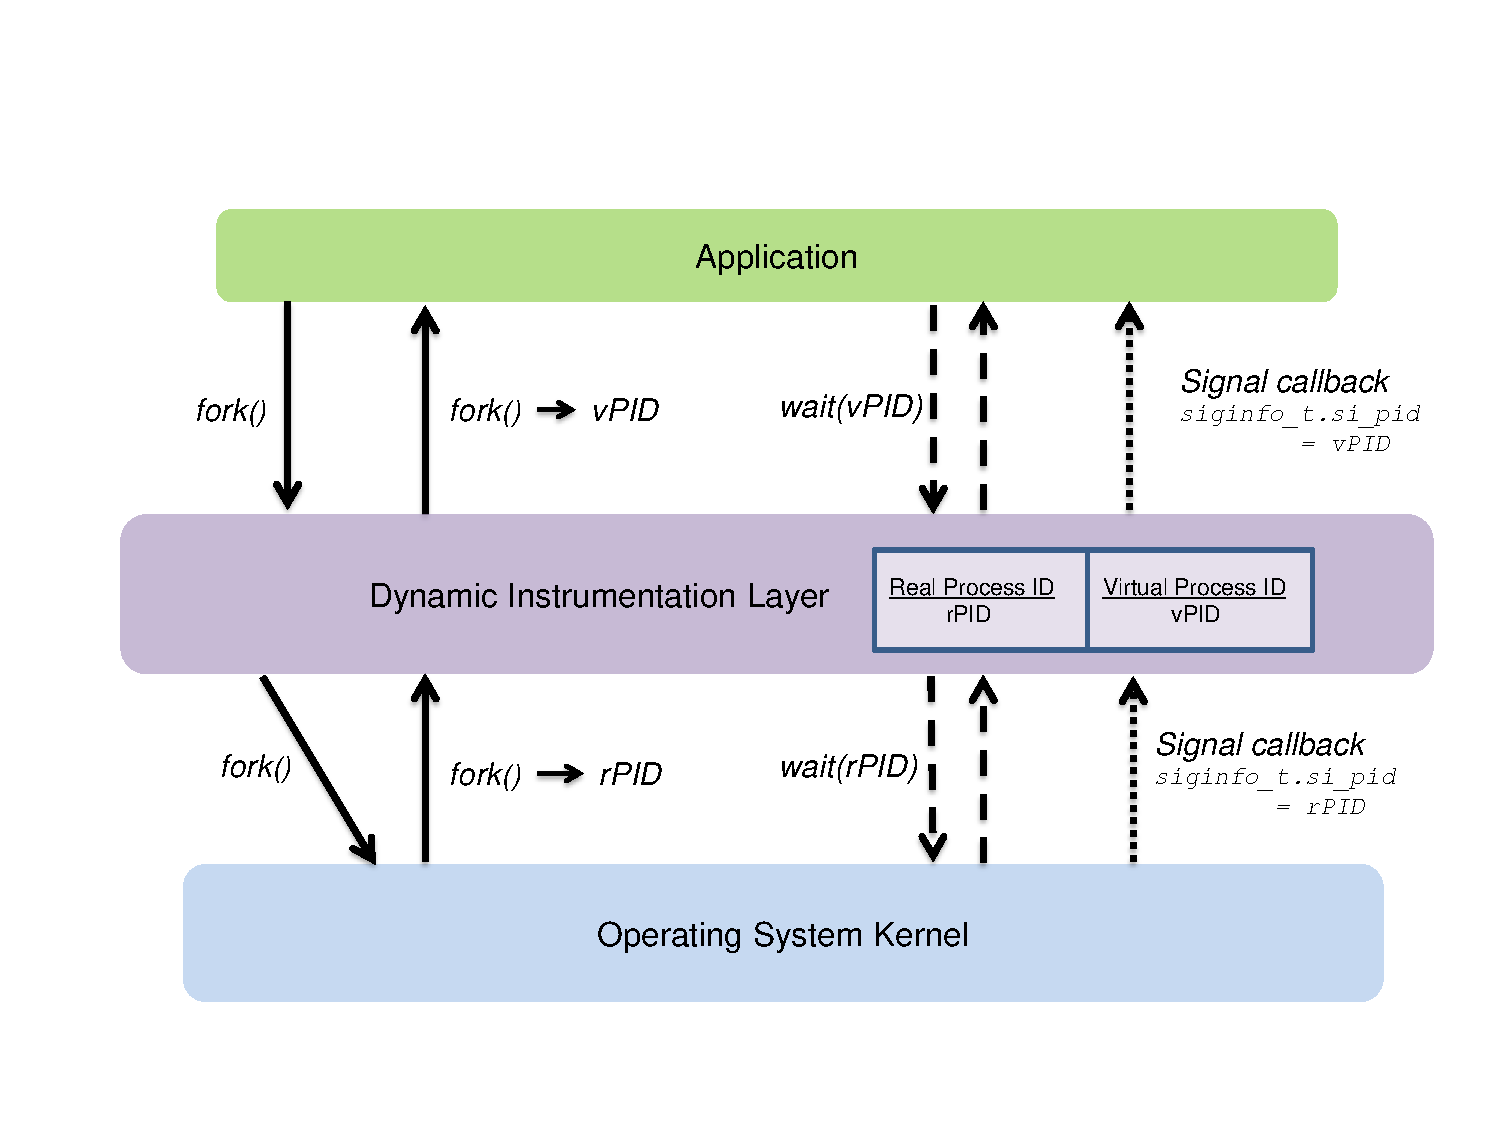
\includegraphics[trim=0cm 1cm 0cm 0.5cm, scale=0.60]{pid.pdf}
  \caption[Virtualizing the process ID layer using Pin]% 
  {All system calls and communications
  between the Linux user and kernel space are intercepted; 
  the dynamic instrumentation layer
  uses a PID translation table, and
  translates between real and virtual process IDs
  to ensure correctness. }
  
  \label{ch3:pidfig}
\end{figure} 

Using dynamic instrumentation, we can replace
real and unpredictable process IDs from kernel space
with virtual and unpredictable process IDs in user space.
As outlined in Section \ref{ch3:pid}, all interfaces
which use process IDs need to be carefully monitored
so that process IDs can be translated back and forth
for correctness. \newline

\noindent {\bf File I/O} \newline
Semantic differences in file contents across
executions would inevitably cause executions
to diverge, but overcoming nondeterminism arsing
from time, randomization or process ID system-calls
is typically sufficient to ensure that
file contents rarely differ in Linux services,
if at all. Some files that may differ
between two instances on start-up (e.g. 
cache files or logs) can simply be 
deleted or replaced without sacrificing correctness.
Also, as mentioned already, \texttt{stat} 
timestamps are frequently not read, so
they can be replaced with fixed constants;
when they are read and only compared with other
\texttt{stat} timestamps, they can be replaced with 
ordinal numbers that perserve ordering;  
otherwise, \texttt{stat} system-calls 
can be faithfully replayed. \newline

\noindent{\bf Network I/O} \newline
The content of network configuration files
does not differ between our identical VMs, so the strategies 
described to handle timestamp comparisons are sufficient
to eliminate nondeterminism from network configuration files.
 
Whenever addresses resolved by various instances differ
between executions, because of DNS-based dynamic load balancing, 
we can intercept and replace resolved IPs with those
stored in the execution signature file.

If the contents read from sockets vary across different executions,
dynamic instrumentation can be used to intercept Linux socket calls
and modify their side-effects to be identical. If
many concurrent executions are reading data from the
same network source, this simply simulates the possibility that all instances
see the same results as the first instance. 

While these semantics are sufficient for most Linux services,
we have not needed to use them: in our experiments,
we have only observed nondeterminism from \texttt{Netlink}
sockets. The techniques used to handle
process IDs and timestamps overcome nondeterminism
in \texttt{Netlink} headers (for source/destination IDs
or sequence numbers). To handle
nondeterminsm from interface statistics
included in \texttt{RTM\_NEWLINK} packets,
we can simply overwrite them with fixed
numbers. 

We can mask nondeterminism from ephemeral ports, 
by changing arguments for \texttt{bind} or \texttt{connect} 
system calls to explicitly request ports
in the ephemeral range rather than letting the kernel 
assign them; alternatively,
we can also virtualize ephemeral ports
similar to how we virtualize process IDs. \newline

\newpage
\noindent{\bf Scalable I/O Schemes} \newline
To handle nondeterminism caused by unpredictable
ordering of I/O ``events'',
we use techniques similar to those used 
for reordering signals,
as described by Figure \ref{ch3:reorderfig}.

\begin{figure}[h]
  \center
  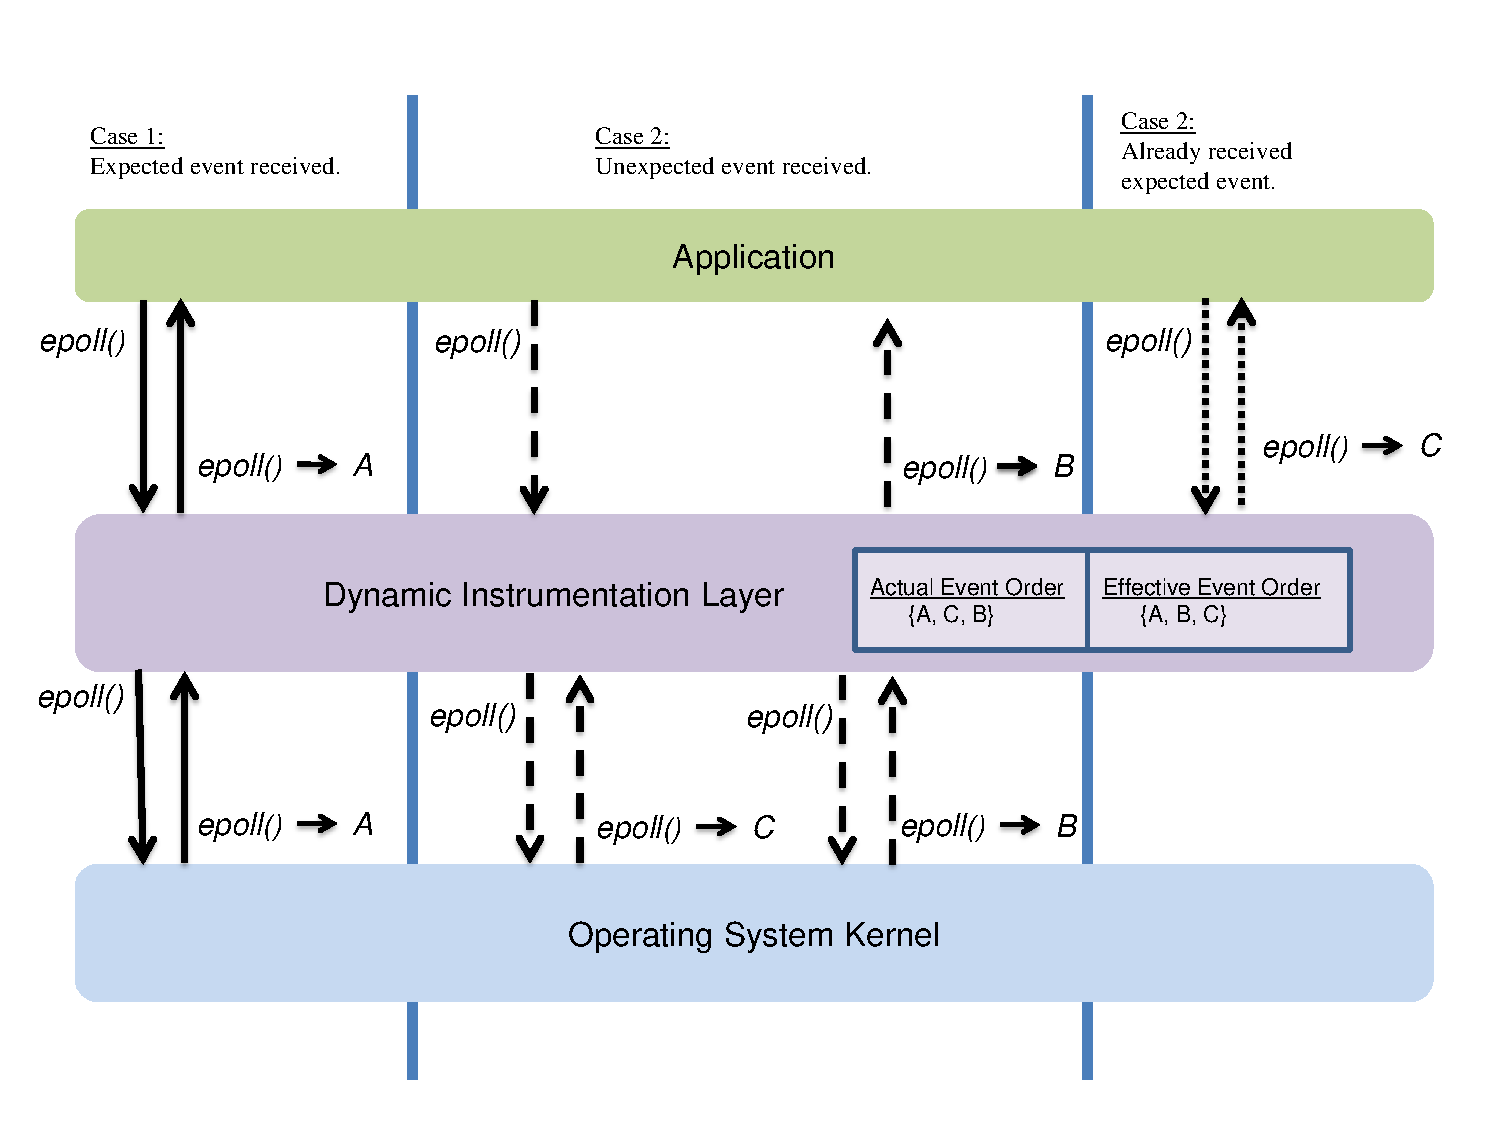
\includegraphics[trim=0cm 0cm 0cm 0cm, scale=0.60]{epoll.pdf}
  \caption[Reordering I/O events using Pin]% 
    {We intercept all \texttt{epoll} system calls,
    and use the execution signature file to
    achieve determinism. We do not ``replay'' I/O
    events because only events that actually do occur
    are delivered to the application instance. This
    diagram assumes \texttt{epoll} returns one event
    per call for the sake of illustration. }       
  \label{ch3:reorderfig}
\end{figure} 
              
Assuming that \texttt{epoll} returns just one event, figure
\ref{ch3:reorderfig} illustrates three possible cases that could occur:
\begin{itemize}
    \item The event returned by a call to \texttt{epoll} is the one expected
    in the execution signature file. The instrumentation layer
    does not modify the system call.
    \item Instead of the expected event,
    \texttt{epoll} returns another event.
    The instrumentation layer stores all such out-of-order events,
    and repeatedly calls \texttt{epoll} until the 
    the expected event is received.
    \item  A call to \texttt{epoll} is initiated, and the
    event returned has already been received.
    The instrumentation layer does not 
    make a system call but simulates a return
    from \texttt{epoll} with the expected event.
\end{itemize}

Even if I/O events are reordered,
it is possible that different amounts
of data are available for a ``ready''
file descriptor for each event
across executions. We can use
dynamic instrumentation to mask
this nondeterminism: if more bytes
are available (e.g. through \texttt{read}) 
than exected in the execution signature
file, we modify return values and \texttt{read}
buffers to delay the reading of these bytes
until the next \texttt{read}. (In some corner
cases, we may have to ``fake'' readiness
if all bytes to be read were available in an event
and we hid them). If less-than-expected
bytes are available, we simply wait
till they are available by waiting for
another readiness update inside 
dynamic instrumentation layer.
In our experiments, this approach has been sufficient to 
achieve deterministic execution.
For asynchronous I/O schemes, schemes
similar to those used for reordering
and timing signals 
would be necessary to hide
the variability of I/O latency.
\newline

\noindent {\bf Concurrency} \newline
Nondeterminism due to multi-threading
has been extensively documented; there
is a significant body of work that
attempts to overcome such nondeterminism
by using deterministic logical clocks
or record-and-replay approaches. 
For our experiments, we did not attempt to enforce
a total order on the instructions executed in multi-threaded
programs and just measured nondeterminism inside 
the main process for each Linux service.
To overcome nondeterminism caused
by multi-threading, we could incorporate
deterministic logical clocks 
into our design by augmenting the
execution signature file.

Similarly, a nondeterministic system scheduler
can cause variable timing of signals
or I/O events, which
can be handled as described previously.
Work on deterministic
operating systems can
be extended to overcome this issue
in a more systematic manner. \newline

\noindent {\bf {\em Procfs}: The \texttt{`/proc/directory'}} \newline
We intercept and modify reads 
from {\em procfs} if necessary. We can simply 
replay reads from {\em procfs} using the execution signature
file, or replace any statistics with fixed and 
reasonable values. We must also intercept
all \texttt{open} system calls with paths
of the form \texttt{`proc/[PID]'},
and switch real and virtual process IDs
in these paths.

\section{Results after Using Deterministic Execution} \label{ch3:data}
We were able to achieve {\em fully} deterministic execution (i.e.
user-mode execution traces that were 100\% identical) in several
Linux services including \texttt{cron}, \texttt{ntp} and
\texttt{cups} using these approaches.

The next chapter describes the context in which nondeterminism
occured in these services and the relative signficance of the various factors we have outlined 
as sources of nondeterminism in programs.

\section{Disadvantages of Deterministic Execution} \label{ch3:issues}
There are several drawbacks and limitations associated with the approach we used
to make execution deterministic:
\begin{itemize}

\item {\em Security:} \newline
Disabling ASLR increases the vulnerability of
applications to external attacks. 
Although canary and pointer guard
values are still dynamically chosen in
our brand of deterministic execution, 
they must agree across all VMs. Thus,
an adversary  who can compromise one VM by
guessing its canary could easily attack the others.
However, the fact that we can choose different
canary or guard values between different bootstorms
still provides some security from these features.

\item {\em Randomization:} \newline
Randomization can be essential for security (e.g. random values
are used to generate keys and certificates),
performance, and sometimes simply correctness (e.g. 
clients may choose random IDs for themselves).
Making PRNG seeds across different instances
agree might impact the security, performance
or correctness of target programs. 

Thankfully, we have not yet discovered any such
issues in the Linux services. Technically,
our approach simulates the extremely unlikely 
-- yet possible -- scenario that all concurrently executing
instances somehow generated the same seeds
from external sources.

\item{\em Time Correctness:} \newline
Any programs that rely on precise
measurements of time (e.g. through \texttt{rdtsc})
will lose correctness. None 
of the services or daemons we considered 
had such an issue.

However, some Linux services (e.g. \texttt{ntp}) 
do rely on measuring time in an accurate 
manner to synchronize the system clock.
Our semantics can cause such services to 
behave incorrectly at start up,
because we do not allow programs to accurately measure time.
However, this is still not a huge correctness problem because these
programs are self-healing. After the booting process is over,
and all VMs branch in execution, \texttt{ntp} will synchronize
the current time correctly.

\item{\em I/O aggregation in Network} \newline
When socket \texttt{read}s return different bytes,
these could be because of synthetic differences (e.g.
in timestamps in headers), or because of 
semantic differences (e.g. different requests or data).
We can study application code and use dynamic instrumentation
to reconstruct network packets and overcome synthetic nondeterminism
from such sources. In our experiments, we used this approach
for \texttt{Netlink} packets, but generalizing it
to all network sockets and protocols, while possible, would clearly
complicate the design of the dynamic instrumentation
layer. For semantic differences in I/O, 
execution would have to branch out.

One possible approach for fixing nondeterminism from external
socket \texttt{reads} would be to forcibly
conform these reads to be identical by replaying
them. This approach would work for many 
Linux services and would simulate the possibility
that these services received responses from
an external source at the exact same time containing
the same data. However, these semantics can
also be problematic in terms of correctness e.g. if the network 
response says ``you have the lock!'' we will have issues
by replaying it.

\end{itemize}
\section {Summary}
